\section{クラスタリング実験}

\subsection{実験環境}

実験にはPython3.5を用い,
機械学習のライブラリとしてTensorFlowを用いてアルゴリズムを実装した.
プログラムはmacOS 10.12上で実行した.

\subsection{精度の評価}

クラスタリング精度の評価は以下の3つの指標により行った.
\begin{description}
  \item[ARI; Adjusted Rand Index, 調整ランド指数]~\\
    クラスタの正解ラベルに対してクラスタリング結果の一致度を評価する指標である.1に近づくほどよいクラスタリング結果と言える.
  \item[NMI; Normalized Mutual Information, 正規化相互情報量]~\\
    相互情報量を正規化した指標である.1に近づくほどよいクラスタリング結果と言える.
  \item[Purity]~\\
    生成されたクラスタがどれだけ多数派で占められているかを表す指標である.1に近づくほどよいクラスタリング結果と言える.
\end{description}
これらの指標は,Pythonのライブラリであるscikit-learnで用意されている関数により求めた.

\subsection{2次元空間のクラスタリング}

まず,2次元のデータのクラスタリング結果を比較する.
実験では,2次元空間に\figurenum{fig:2dim}のような分散$\sigma^2=1$の混合等方Gauss分布を用いた.
この混合等方ガウス分布は5つの等方ガウス分布で構成される.
そして,各クラスタは500個のデータ点を持つ.
このデータに対し,対数尤度関数,BIC, AIC, cAICを分割停止規準として採用してX-meansによるクラスタリングを行った.

\tablenum{table:2dim}はX-meansにより推定されたクラスタ数,X-meansにより得られたクラスタリング結果のARI, NMI, Purityを示す.
各データは,100回ランダムに生成されたデータに対してクラスタリングをそれぞれ行ったあと得られた結果の平均であり,括弧内の数値は分散を表す.
\tablenum{table:2dim}より,2次元空間において分割停止規準としてBICとcAICを採用したXmeansの
クラスタリング結果に大きな差がないことが分かった.
どちらの情報量基準を用いたX-meansの結果もクラスタ数の推定もおおよそ出来ており,推定したクラスタ数の分散もあまり大きな値とはなっていない.

また,AICを分割停止規準として採用した場合に着目すると,推定したクラスタ数の分散が非常に大きくなっている.
これは,3.3節で述べたように,AICはクラスタ数を過大に見積もってしまうことに起因すると思われる.
実際に,推定されたクラスタ数を見ると,クラスタ数を20や22と推定しているものが多く存在した.
しかし,対数尤度関数を分割停止規準として採用した場合のクラスタリング結果と比較すると,
比較的安定したクラスタ数推定を行っていることが見て取れる.

\begin{table}[htb]
  \centering
  \caption{2次元空間におけるクラスタリング結果}
  \label{table:2dim}
  \begin{tabular}{|c|c|c|c|c|} \hline
    分割停止規準 & クラスタ数(分散) & ARI & NMI & Purity \\\hline
    BIC & 4.58 (0.9836) & 0.84458792 & 0.88281495 & 0.84458792\\
    cAIC & 4.55 (0.6475) & 0.85329139 & 0.89992544 & 0.85329139\\
    AIC & 4.69 (3.8739) & 0.83642236 & 0.88147442 & 0.83642236\\
    対数尤度関数 & 5.32 (10.236) & 0.85699618 & 0.91572100 & 0.85699618\\\hline
  \end{tabular}
\end{table}

\begin{figure}[htbp]
  \begin{center}
    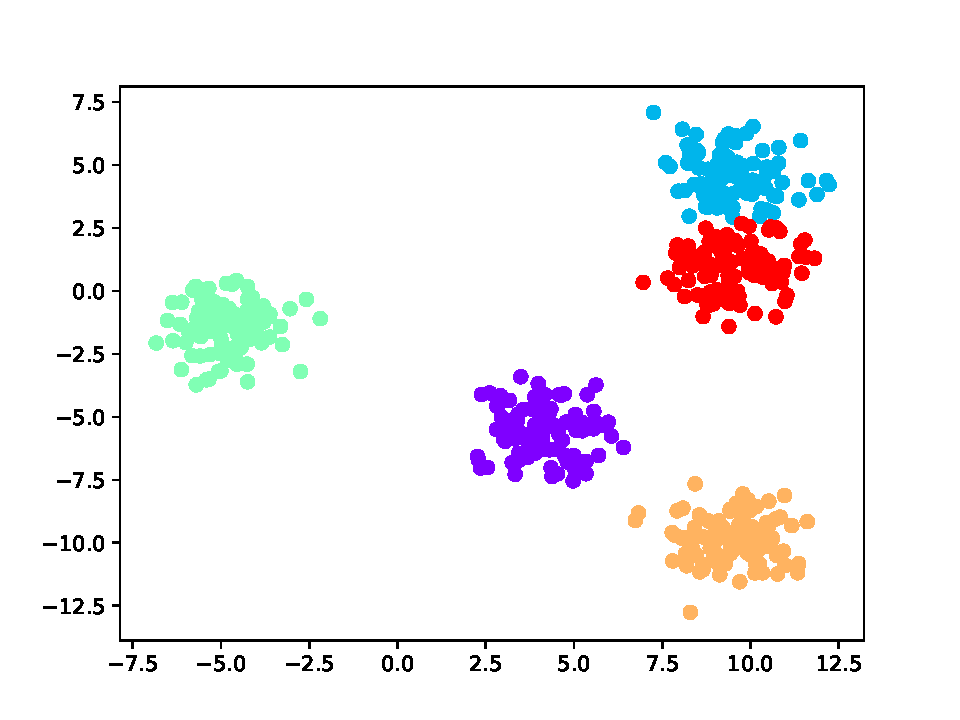
\includegraphics[width=0.7\linewidth]{./img/BIC_2.pdf}
      \caption{2次元空間のクラスタリング例}
      \label{fig:2dim}
  \end{center}
\end{figure}

\subsection{3次元空間のクラスタリング}

3次元空間に\figurenum{fig:3dim}のようにデータを分散$\sigma^2=1$の混合等方Gauss分布より生成した.
実験で使用するデータは図のように5つのクラスタで構成されており,各クラスタは500個のデータ点を持つ.
このデータに対し,対数尤度関数,BIC, AIC, cAICを分割停止規準として採用してクラスタリングを行った.

\begin{figure}[htbp]
  \begin{center}
    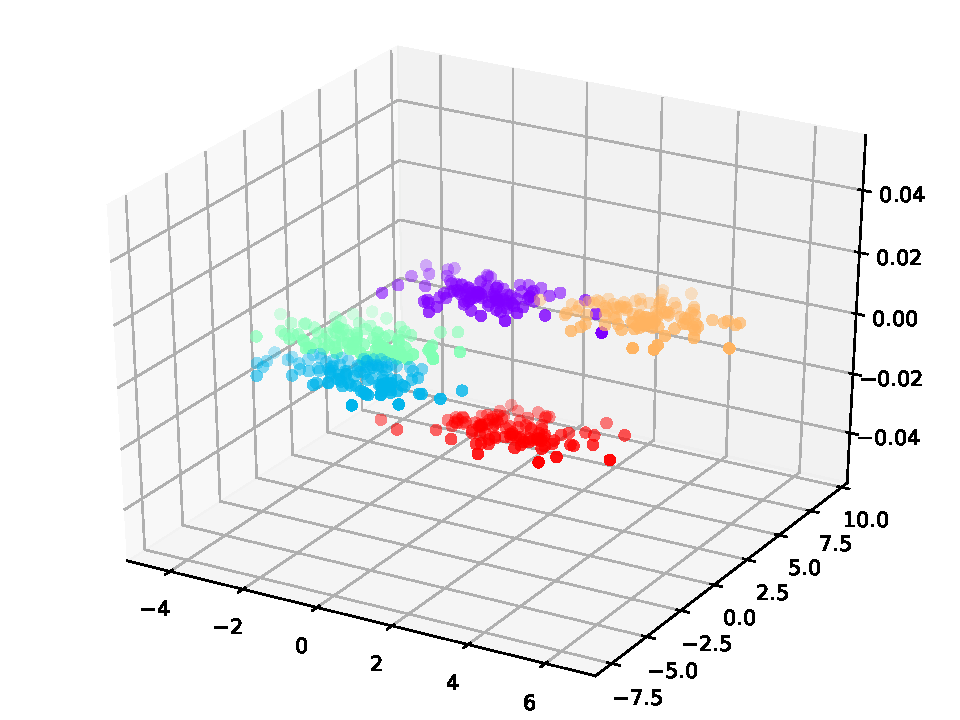
\includegraphics[width=0.7\linewidth]{./img/BIC_3.pdf}
      \caption{3次元空間のクラスタリング例}
      \label{fig:3dim}
  \end{center}
\end{figure}

\tablenum{table:3dim}に都度ランダムに生成されたデータに対して100回クラスタリングを行ったときの,
推定されたクラスタ数,ARI, NMI, Purityの平均値および推定されたクラスタ数の分散を示す.
2次元のクラスタリングとは異なり,3次元空間においてはBICを分割停止規準として採用した場合の精度が良くなっている.
分散値も非常に小さいため,安定して精度の高いクラスタ数推定を行っていることが伺える.

cAICとAICの場合を比較した場合,cAICのほうがクラスタリングの精度が高いことがわかる.
また,AICを用いた場合では,2次元空間ほど推定されたクラスタ数の分散が大きくないことがわかる.
2次元空間では,クラスタ数を過大に見積もってしまう問題があったが,
3次元空間においてその問題は発生していなかった.

\begin{table}[htb]
  \centering
  \caption{3次元空間におけるクラスタリング結果}
  \label{table:3dim}
  \begin{tabular}{|c|c|c|c|c|} \hline
    分割停止規準 & クラスタ数(分散) & ARI & NMI & Purity \\\hline
    BIC & 4.95 (0.0669) & 0.97179074 & 0.97913818 & 0.97179074\\
    cAIC & 4.92 (0.2313) & 0.96312702 & 0.97023920 & 0.96312702\\
    AIC & 4.88 (0.1443) & 0.95216819 & 0.96855698 & 0.95216819\\
    対数尤度関数 & 5.12 (4.1443) & 0.95731637 & 0.96541468 & 0.95731637\\\hline
  \end{tabular}
\end{table}
